% Auriga theme
% https://github.com/anishathalye/auriga

\documentclass[14pt,aspectratio=169]{beamer}
\usepackage{pgfpages}
\usepackage{fancyvrb}
\usepackage{booktabs,dcolumn}
\usepackage{tikz}
\usetikzlibrary{arrows.meta, positioning, quotes}
\usepackage{pgfplots}

% \ifnotes
% \setbeamertemplate{note page}[plain]
% \setbeameroption{show notes on second screen=right}
% \fi

\usetheme{auriga}
\usecolortheme{auriga}

% define some colors for a consistent theme across slides
\definecolor{red}{RGB}{181, 23, 0}
\definecolor{blue}{RGB}{0, 118, 186}
\definecolor{gray}{RGB}{146, 146, 146}

\title{Historia Económica Argentina}

\author{\underline{Sebastián Freille} \inst{1}}

\institute[shortinst]{\inst{1} IEF-UNC \\ UCC}
\date{}

\AtBeginSection[]{
    \begin{frame}
    \vfill
    \centering
    \begin{beamercolorbox}[sep=8pt,center,shadow=true,rounded=true]{title}
        \usebeamerfont{title}\insertsectionhead\par%
    \end{beamercolorbox}
    \vfill
    \end{frame}
}


\AtBeginSubsection[]{
    \begin{frame}
    \vfill
    \centering
    \begin{beamercolorbox}[sep=6pt,center,shadow=true,rounded=true]{title}
        \usebeamerfont{title}\insertsubsectionhead\par%
    \end{beamercolorbox}
    \vfill
    \end{frame}
}


\AtBeginSubsubsection[]{
    \begin{frame}
    \vfill
    \centering
    \begin{beamercolorbox}[sep=4pt,center,shadow=true,rounded=true]{title}
        \usebeamerfont{title}\insertsubsubsectionhead\par%
    \end{beamercolorbox}
    \vfill
    \end{frame}
}



\begin{document}
\maketitle

{
  % rather than use the frame options [noframenumbering,plain], we make the
  % color match, so that the indicated page numbers match PDF page numbers
  \setbeamercolor{page number in head/foot}{fg=background canvas.bg}
  \begin{frame}
    \titlepage
  \end{frame}
}


\section{Capítulo 1.  El período de progreso (1880-1914)}


\subsection{Contexto}


\begin{frame}\frametitle{Series de largo plazo}
\begin{figure}[htbp]\vspace{-0.1cm}
  \centering
  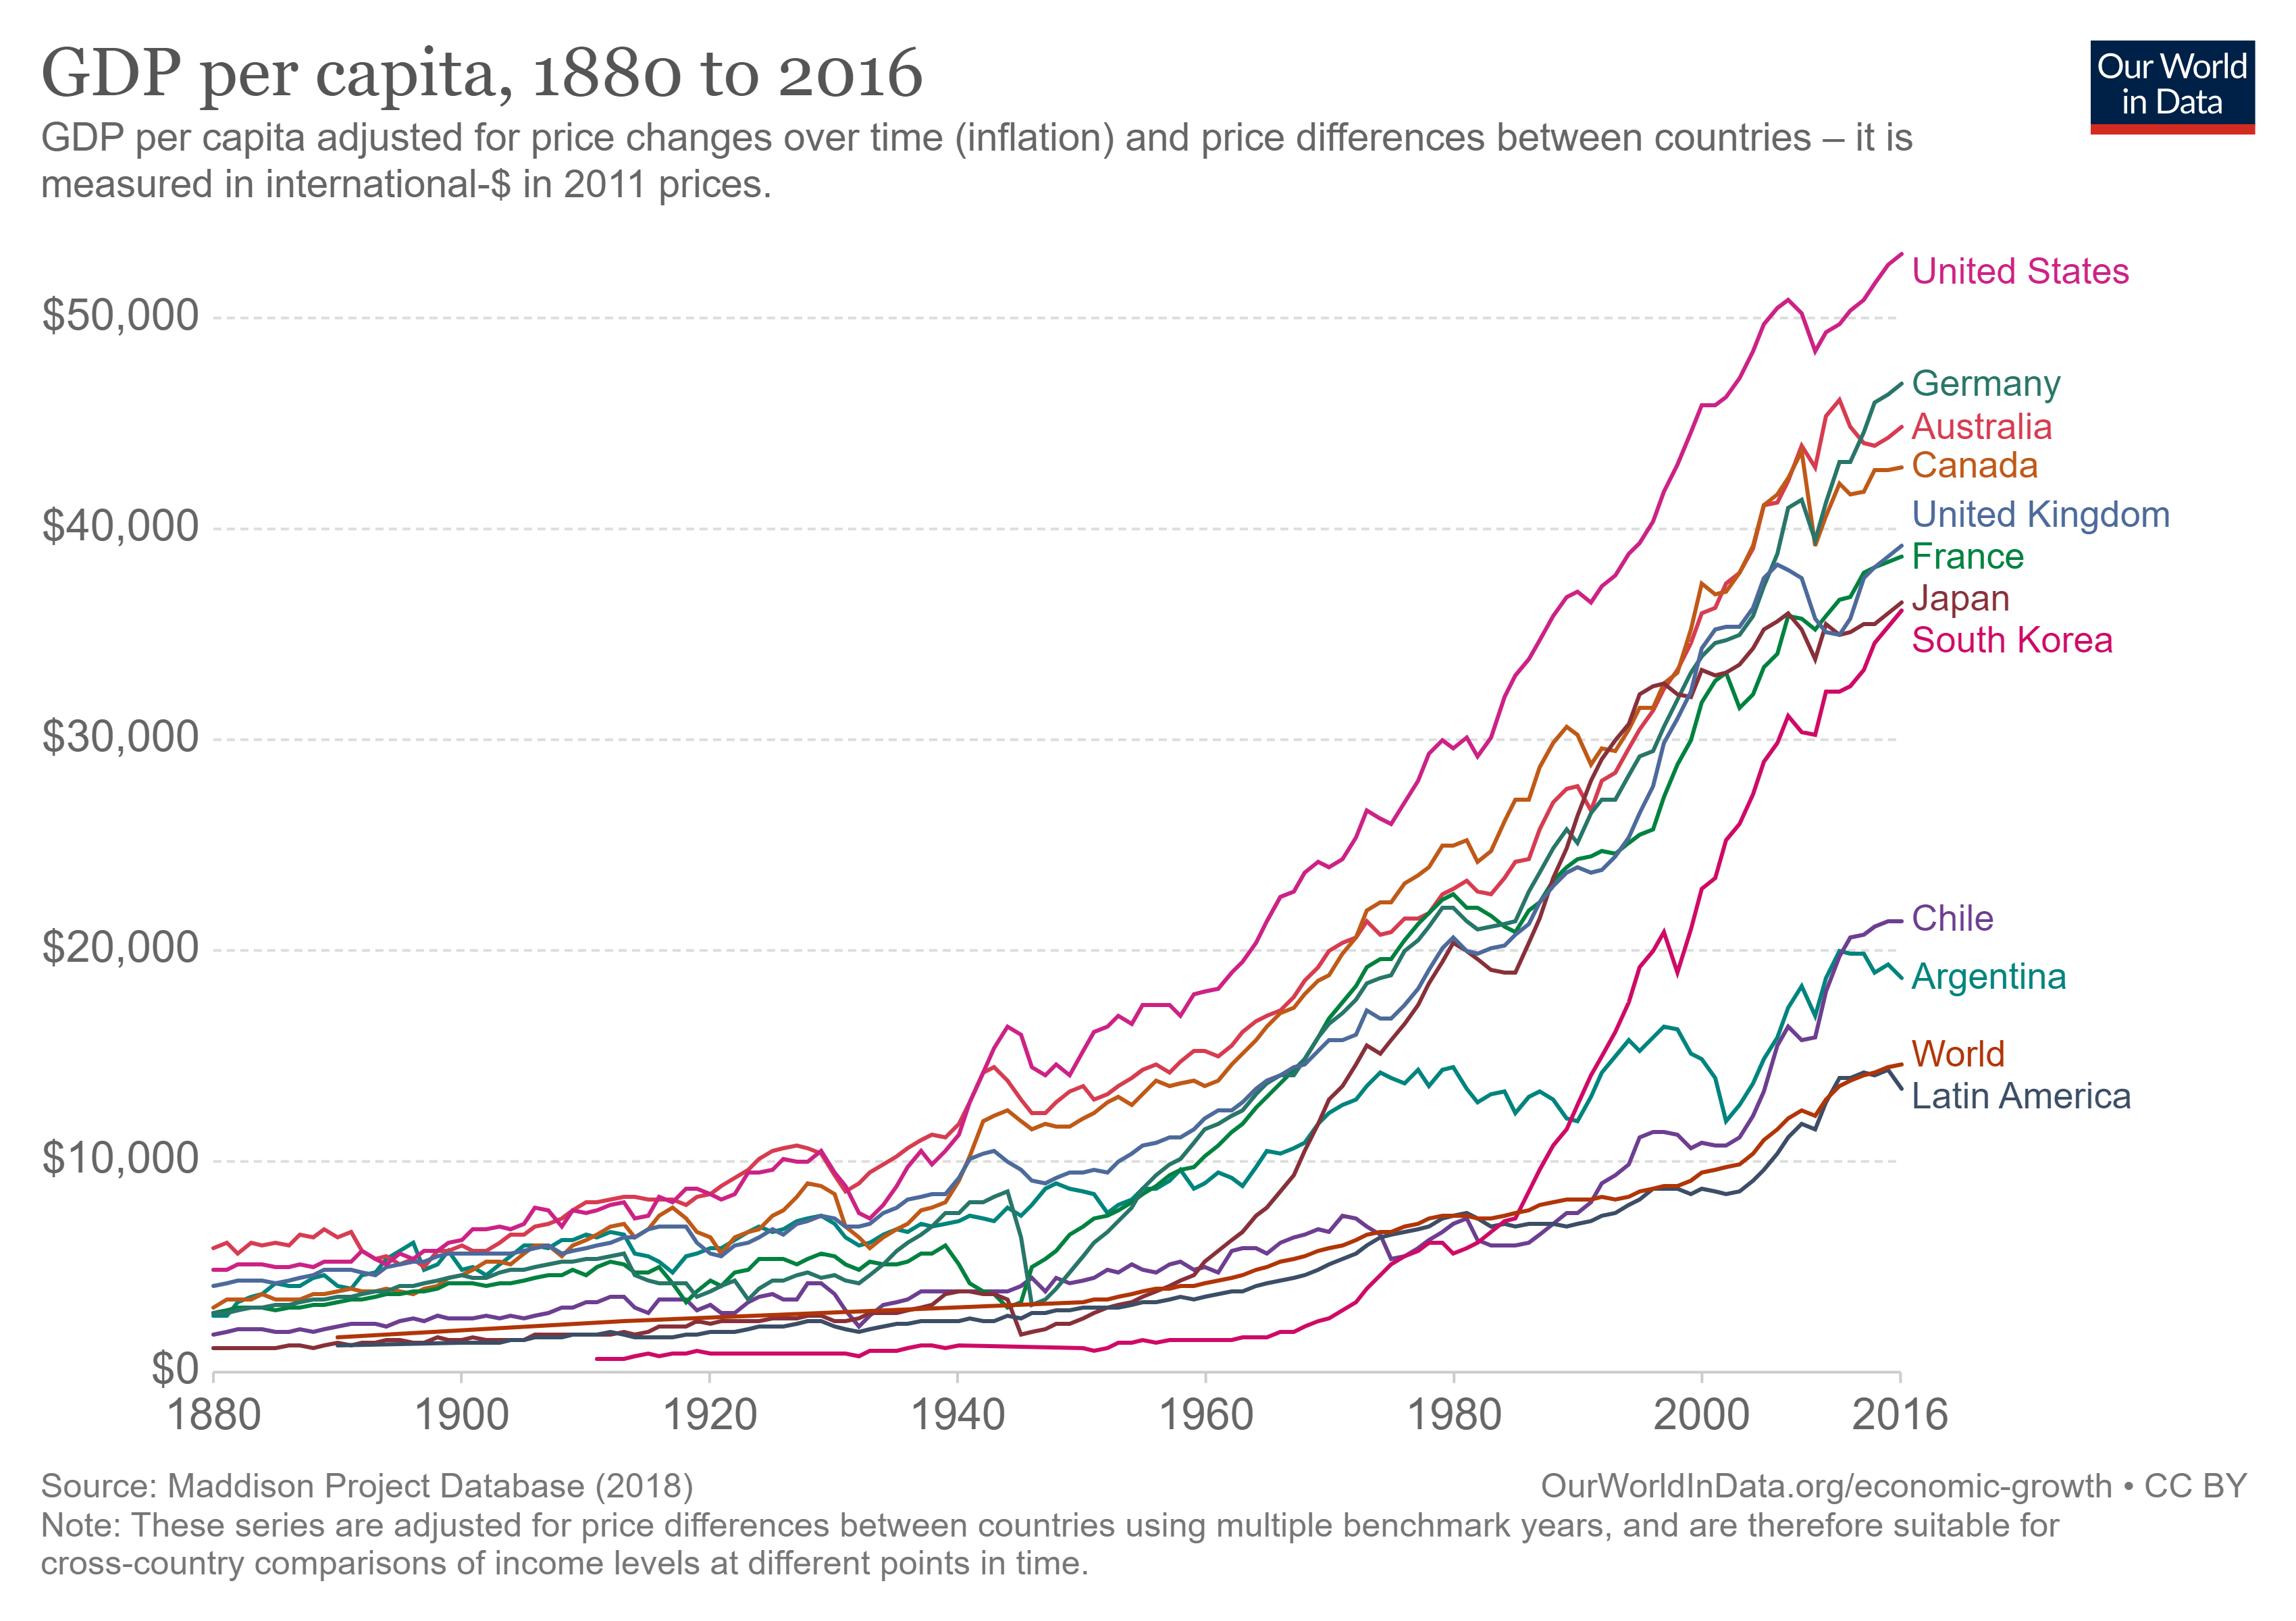
\includegraphics[scale=0.085]{maddison-data-gdp-per-capita-in-2011us-1880-2016}
  \caption[bpe]{Desempeño económico a largo plazo }
  \label{fig:uni1_01}
\end{figure} 
\end{frame}

\begin{frame}\frametitle{Series de largo plazo (cont.)}
\vspace{-0.5cm}
    \begin{columns}
       \begin{column}{0.33\linewidth}\vspace{-0.25cm}
      \begin{figure}
        \centering
        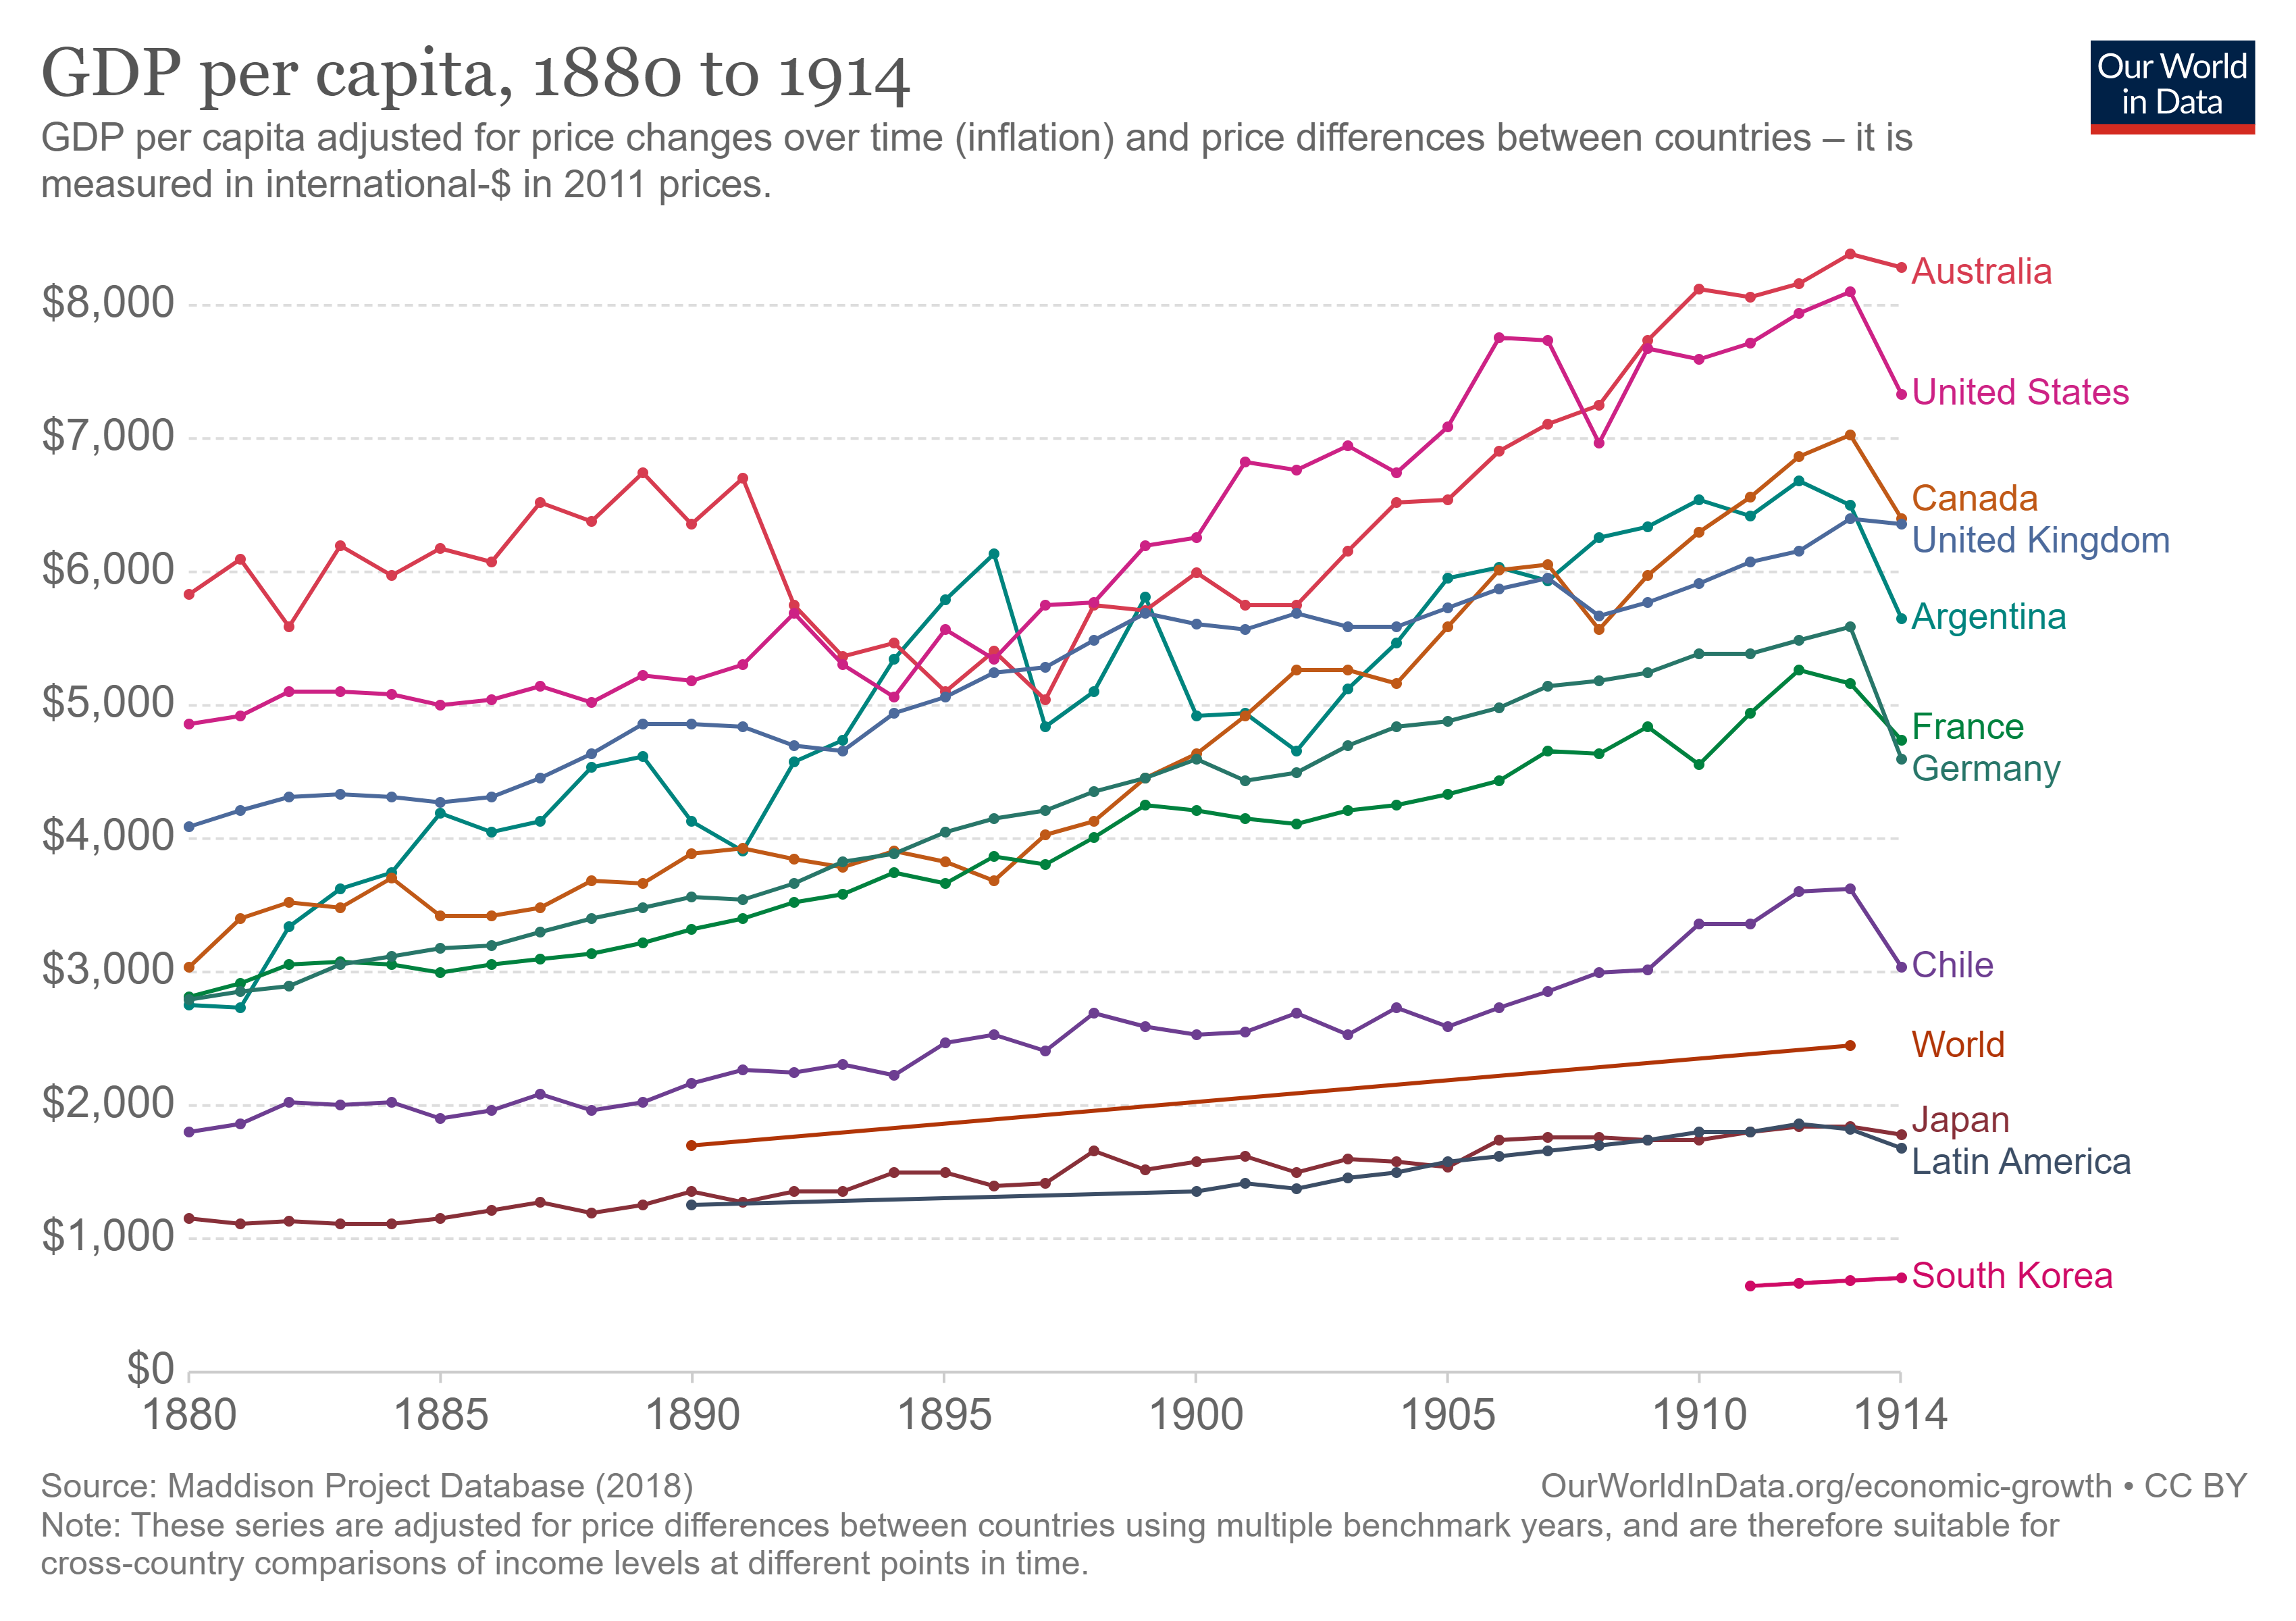
\includegraphics[scale=0.04]{maddison-data-gdp-per-capita-in-2011us-1880-1914}
        %\caption{Crecimiento argentino comparado: 1880-1914}
      \end{figure}
    \end{column}
 \begin{column}{0.33\linewidth}\vspace{-0.25cm}
      \begin{figure}
        \centering
        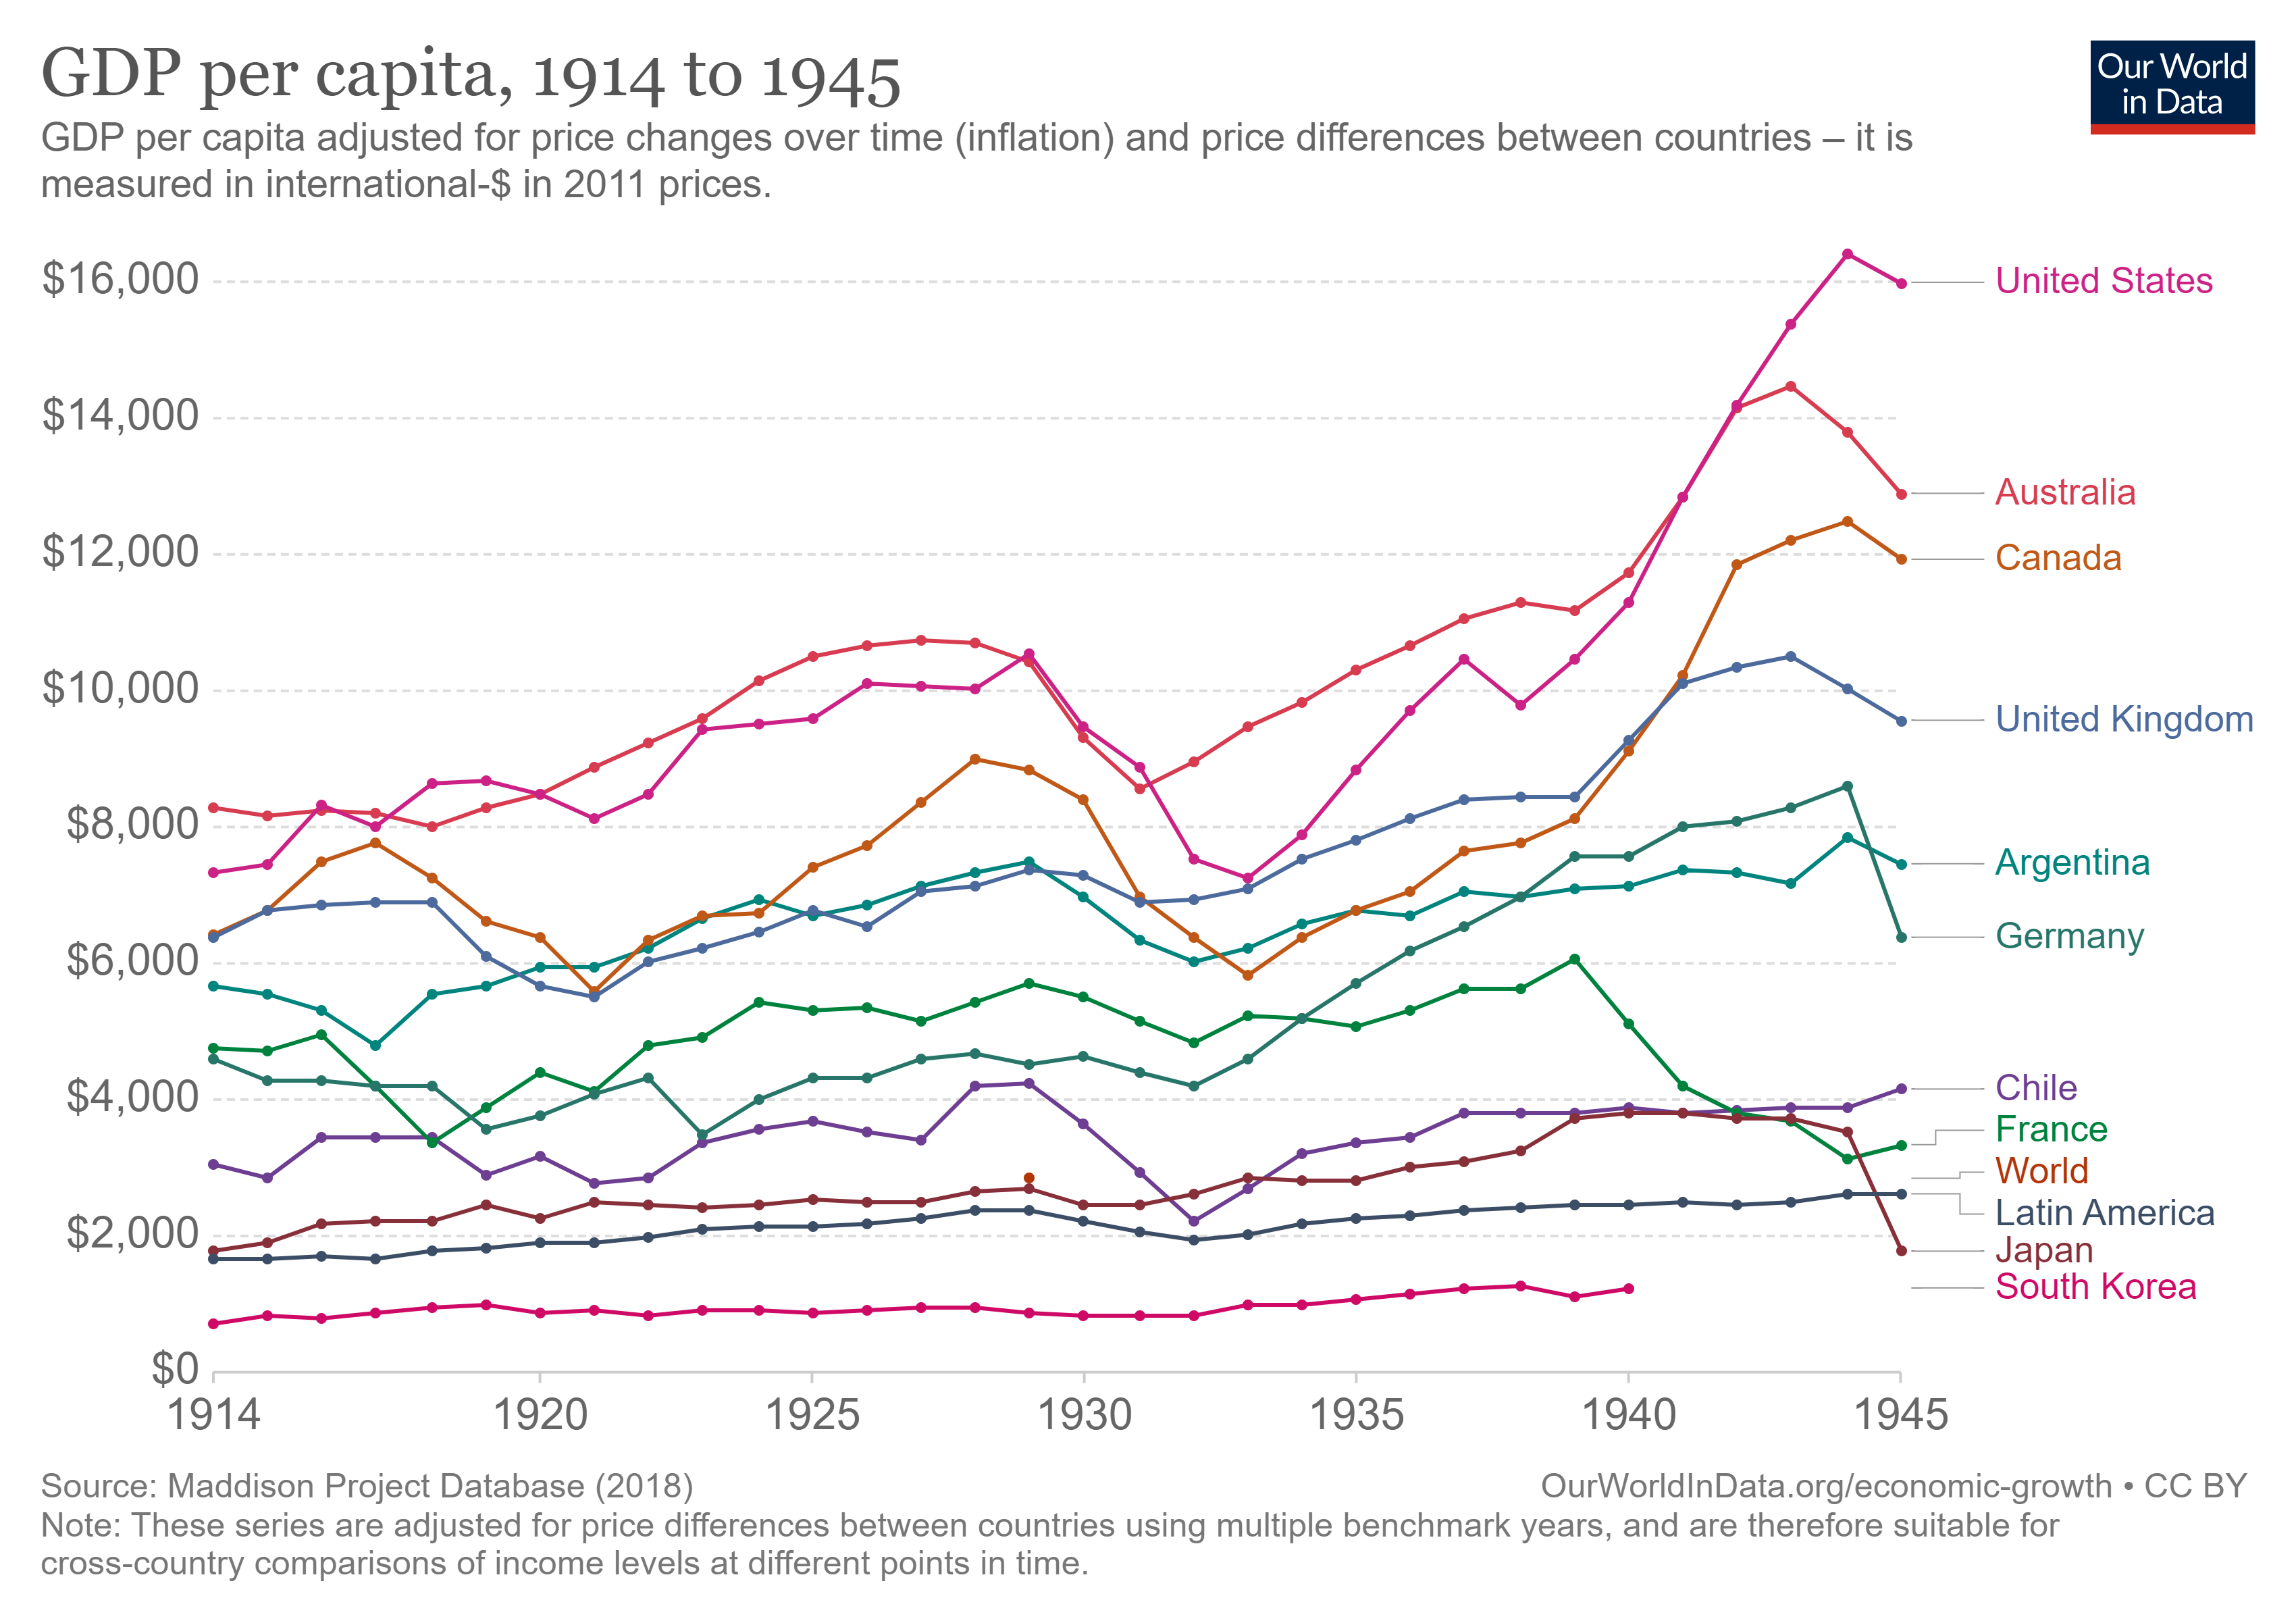
\includegraphics[scale=0.04]{maddison-data-gdp-per-capita-in-2011us-1914-1945}
        %\caption{Crecimiento argentino comparado: 1880-1914}
      \end{figure}
    \end{column}
 \begin{column}{0.33\linewidth}\vspace{-0.25cm}
        \begin{figure}
        \centering
        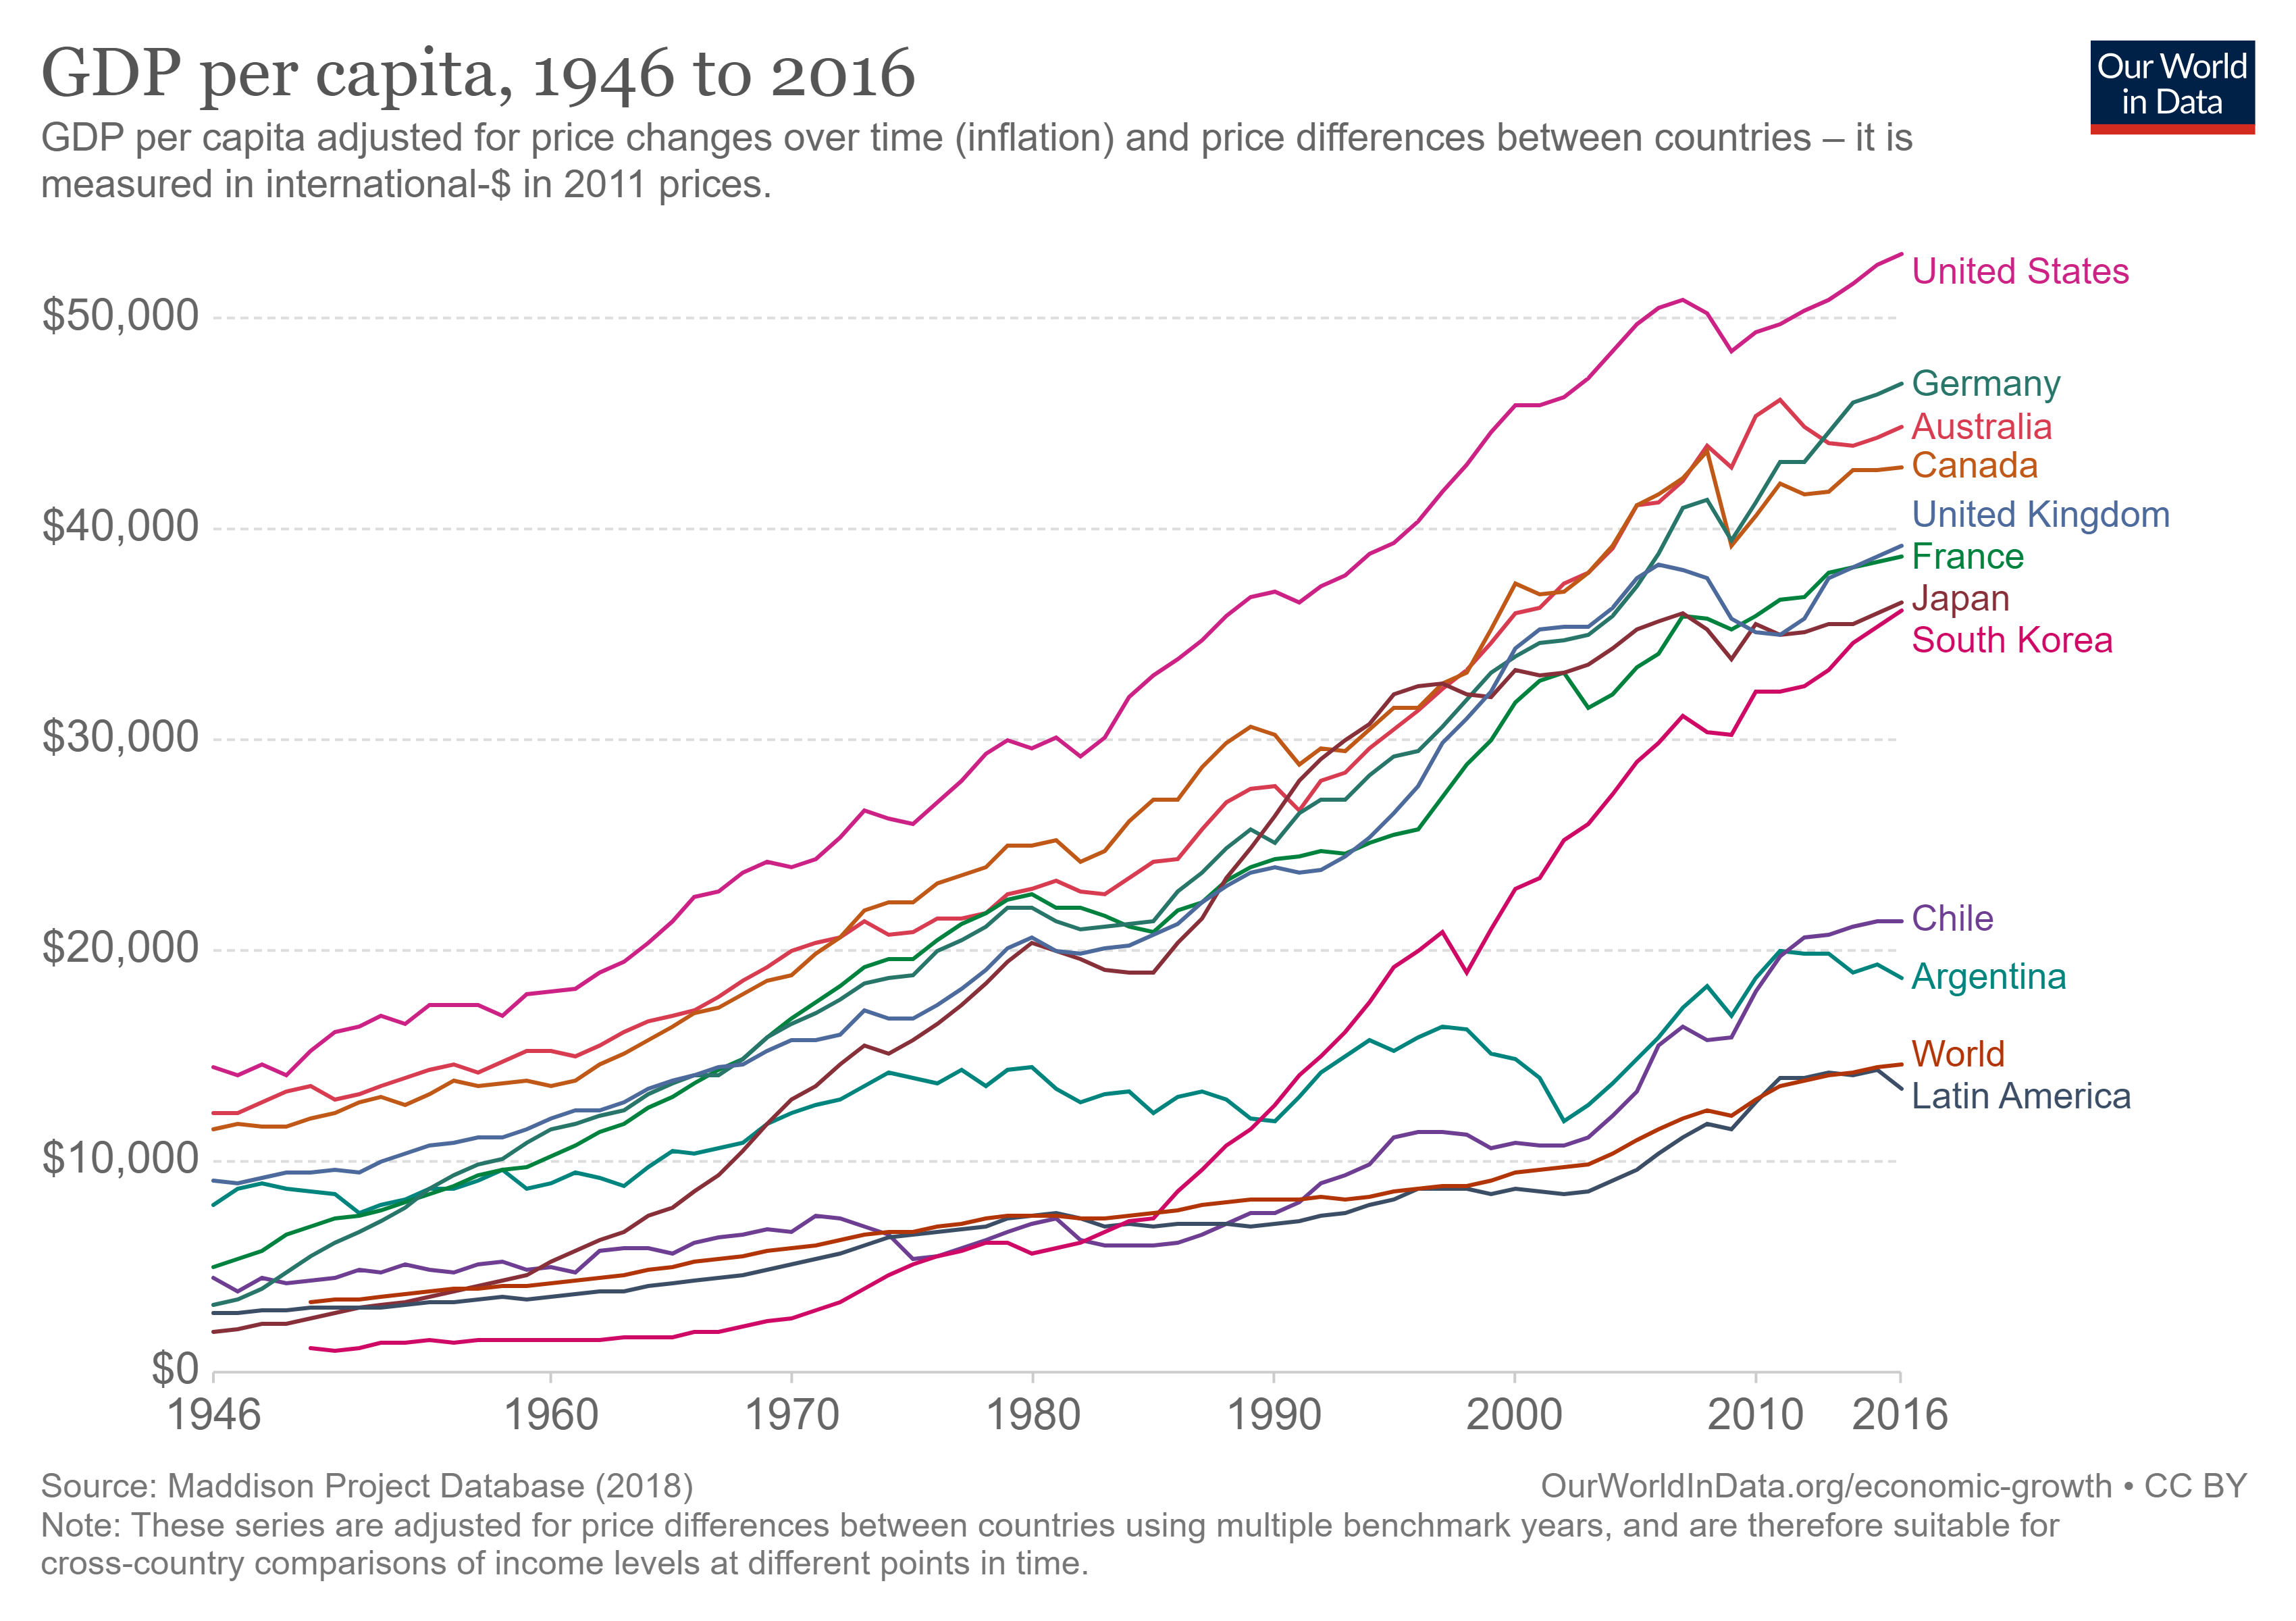
\includegraphics[scale=0.04]{maddison-data-gdp-per-capita-in-2011us-1946-2016}
        %\caption{Crecimiento argentino comparado: 1880-1914}
      \end{figure}
    \end{column}
  \end{columns}
  \end{frame}


\begin{frame}\frametitle{Series de largo plazo (cont.)}
\begin{figure}[htbp]\vspace{-0.1cm}
  \centering
  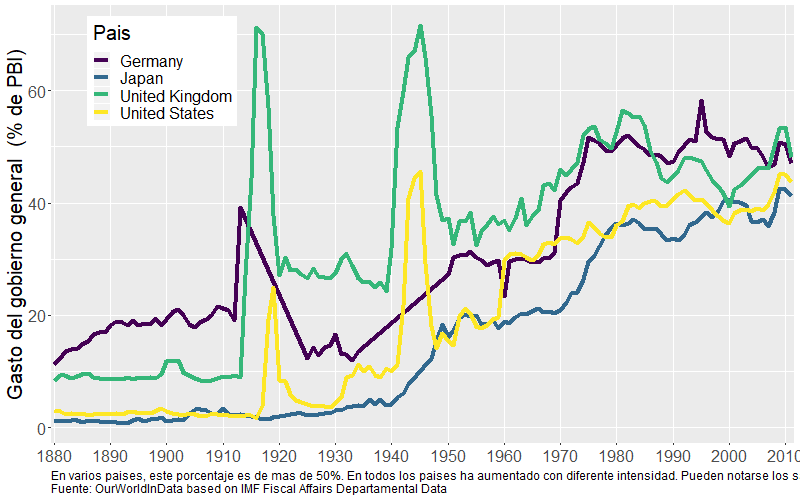
\includegraphics[scale=0.4]{fig03}
  \caption[bpe]{Gasto público - Evolución}
  \label{fig:uni1_01}
\end{figure} 
  \end{frame}

\begin{frame}\frametitle{Series de largo plazo (cont.)}
\begin{figure}[htbp]\vspace{-0.1cm}
  \centering
  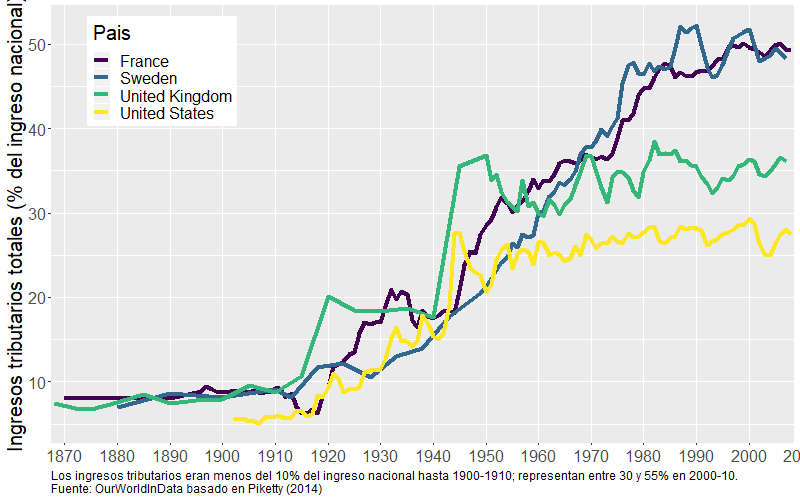
\includegraphics[scale=0.4]{fig04}
  \caption[bpe]{Recursos tributarios - Evolución}
  \label{fig:uni1_01}
\end{figure} 
  \end{frame}


  \begin{frame}\frametitle{Series de largo plazo (cont.)}
\begin{figure}[htbp]\vspace{-0.1cm}
  \centering
  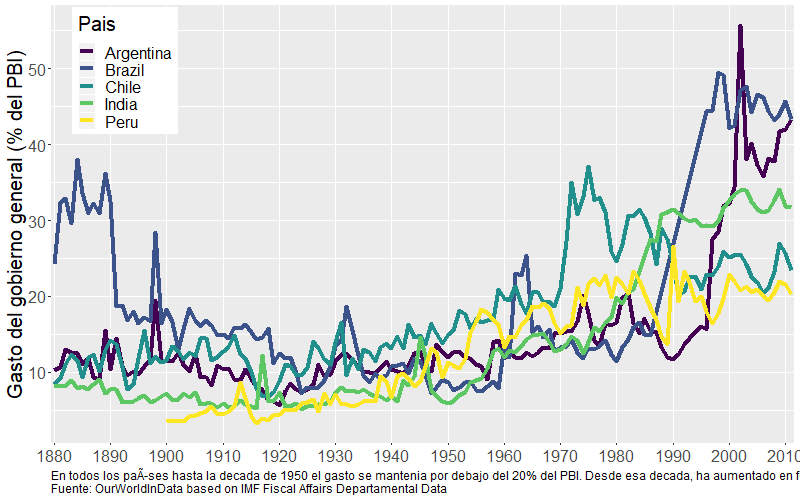
\includegraphics[scale=0.4]{fig05}
  \caption[bpe]{Gasto público - Evolución (otros paises)}
  \label{fig:uni1_01}
\end{figure} 
  \end{frame}


 \begin{frame}\frametitle{Series de largo plazo (cont.)}
\begin{figure}[htbp]\vspace{-0.1cm}
  \centering
  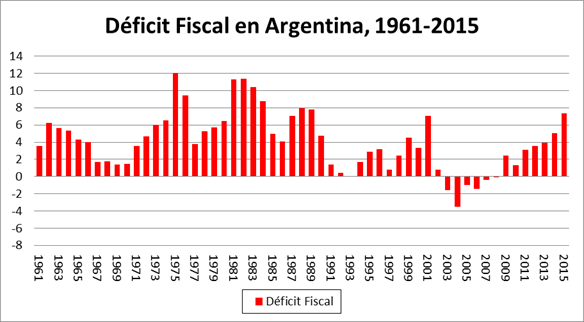
\includegraphics[scale=0.6]{uni8_deficit1}
  \caption[bpe]{Deficit público}
  \label{fig:uni1_01}
\end{figure} 
  \end{frame}
  

  
\subsection{El crecimiento económico (1880-1914)}

\begin{frame}\frametitle{Expansión economica: El período 1880-1914}
     \begin{itemize}
     \item Economía mundial tuvo un gran crecimiento entre
       1880 y 1914. Fuerte aumento del comercio de ByS
       y fenomenal aumento del movimiento de capitales y población
       \item Los principales actores de la economía mundial --UK,
         EEUU, Alemania y Francia-- tenían muy altos niveles de
         ingreso per cápita junto con Australia, Canadá,
         y...Argentina!
         \item ¿Cuáles fueron los factores detrás del gran crecimiento
           argentino en este periodo? $\longrightarrow$ \textbf{teoría
             del bien primario exportable}
         \end{itemize}
        \end{frame}



\begin{frame}\frametitle{Expansión economica: El período 1880-1914 (cont.)}
\vspace{-0.5cm}
    \begin{columns}
    \begin{column}{0.5\linewidth}
       \begin{figure}
        \centering
        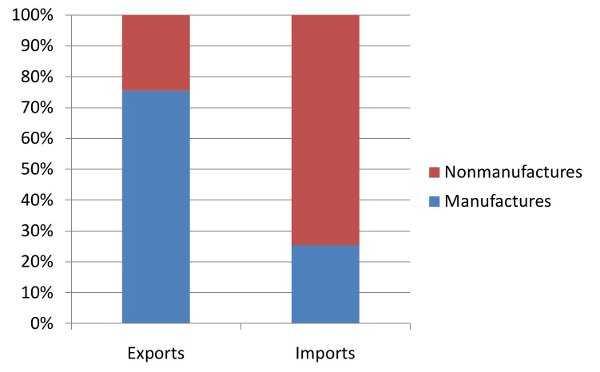
\includegraphics[scale=0.4]{uni1_pattern01}
        \caption{Composición del comercio de UK en 1910s (Fuente:
          Krugman (2008)}
      \end{figure}
    \end{column}
    \begin{column}{0.5\linewidth}
      \begin{figure}
        \centering
        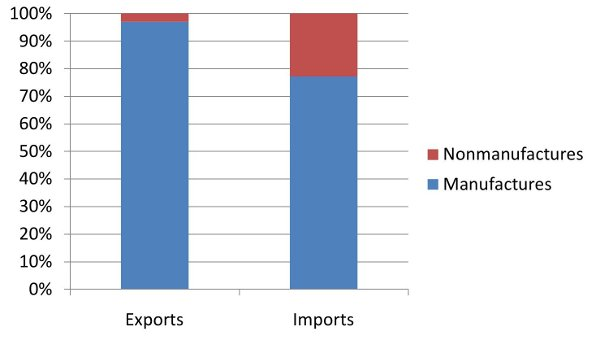
\includegraphics[scale=0.42]{uni1_pattern02}
        \caption{Composición del comercio de UK en 1990s (Fuente:
          Krugman (2008)}
      \end{figure}
    \end{column}
  \end{columns}
  \end{frame}


\begin{frame}\frametitle{Expansión economica: El período 1880-1914 (cont.)}
\vspace{-0.5cm}
    \begin{columns}
    \begin{column}{0.4\linewidth}
      \begin{itemize}
        \item Comercio bilateral en 1910 encajaba con
          patrón de la ventaja comparativa clásica
          \item Favorecía a países que pudieran exportar bs primarios
      \end{itemize}
    \end{column}
    \begin{column}{0.6\linewidth}\vspace{-0.25cm}
      \begin{figure}
        \centering
        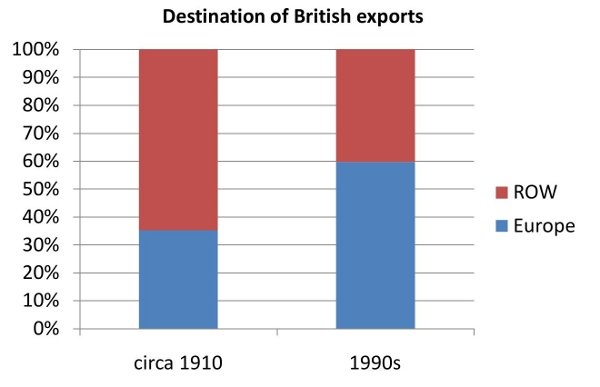
\includegraphics[scale=0.4]{uni1_pattern03}
        %\caption{Crecimiento argentino comparado: 1880-1914}
      \end{figure}
    \end{column}
  \end{columns}
  \end{frame}
  
  
        

\begin{frame}\frametitle{Expansión economica: El período 1880-1914 (cont.)}
\vspace{-0.5cm}
    \begin{columns}
    \begin{column}{0.4\linewidth}
      \begin{itemize}
        \item Entre países con mayor PBI per capita
        \item Sólo Canadá mejor performance que Argentina
          \item Mas volatilidad que US, Canadá y europeos 
      \end{itemize}
    \end{column}
    \begin{column}{0.6\linewidth}\vspace{-0.25cm}
      \begin{figure}
        \centering
        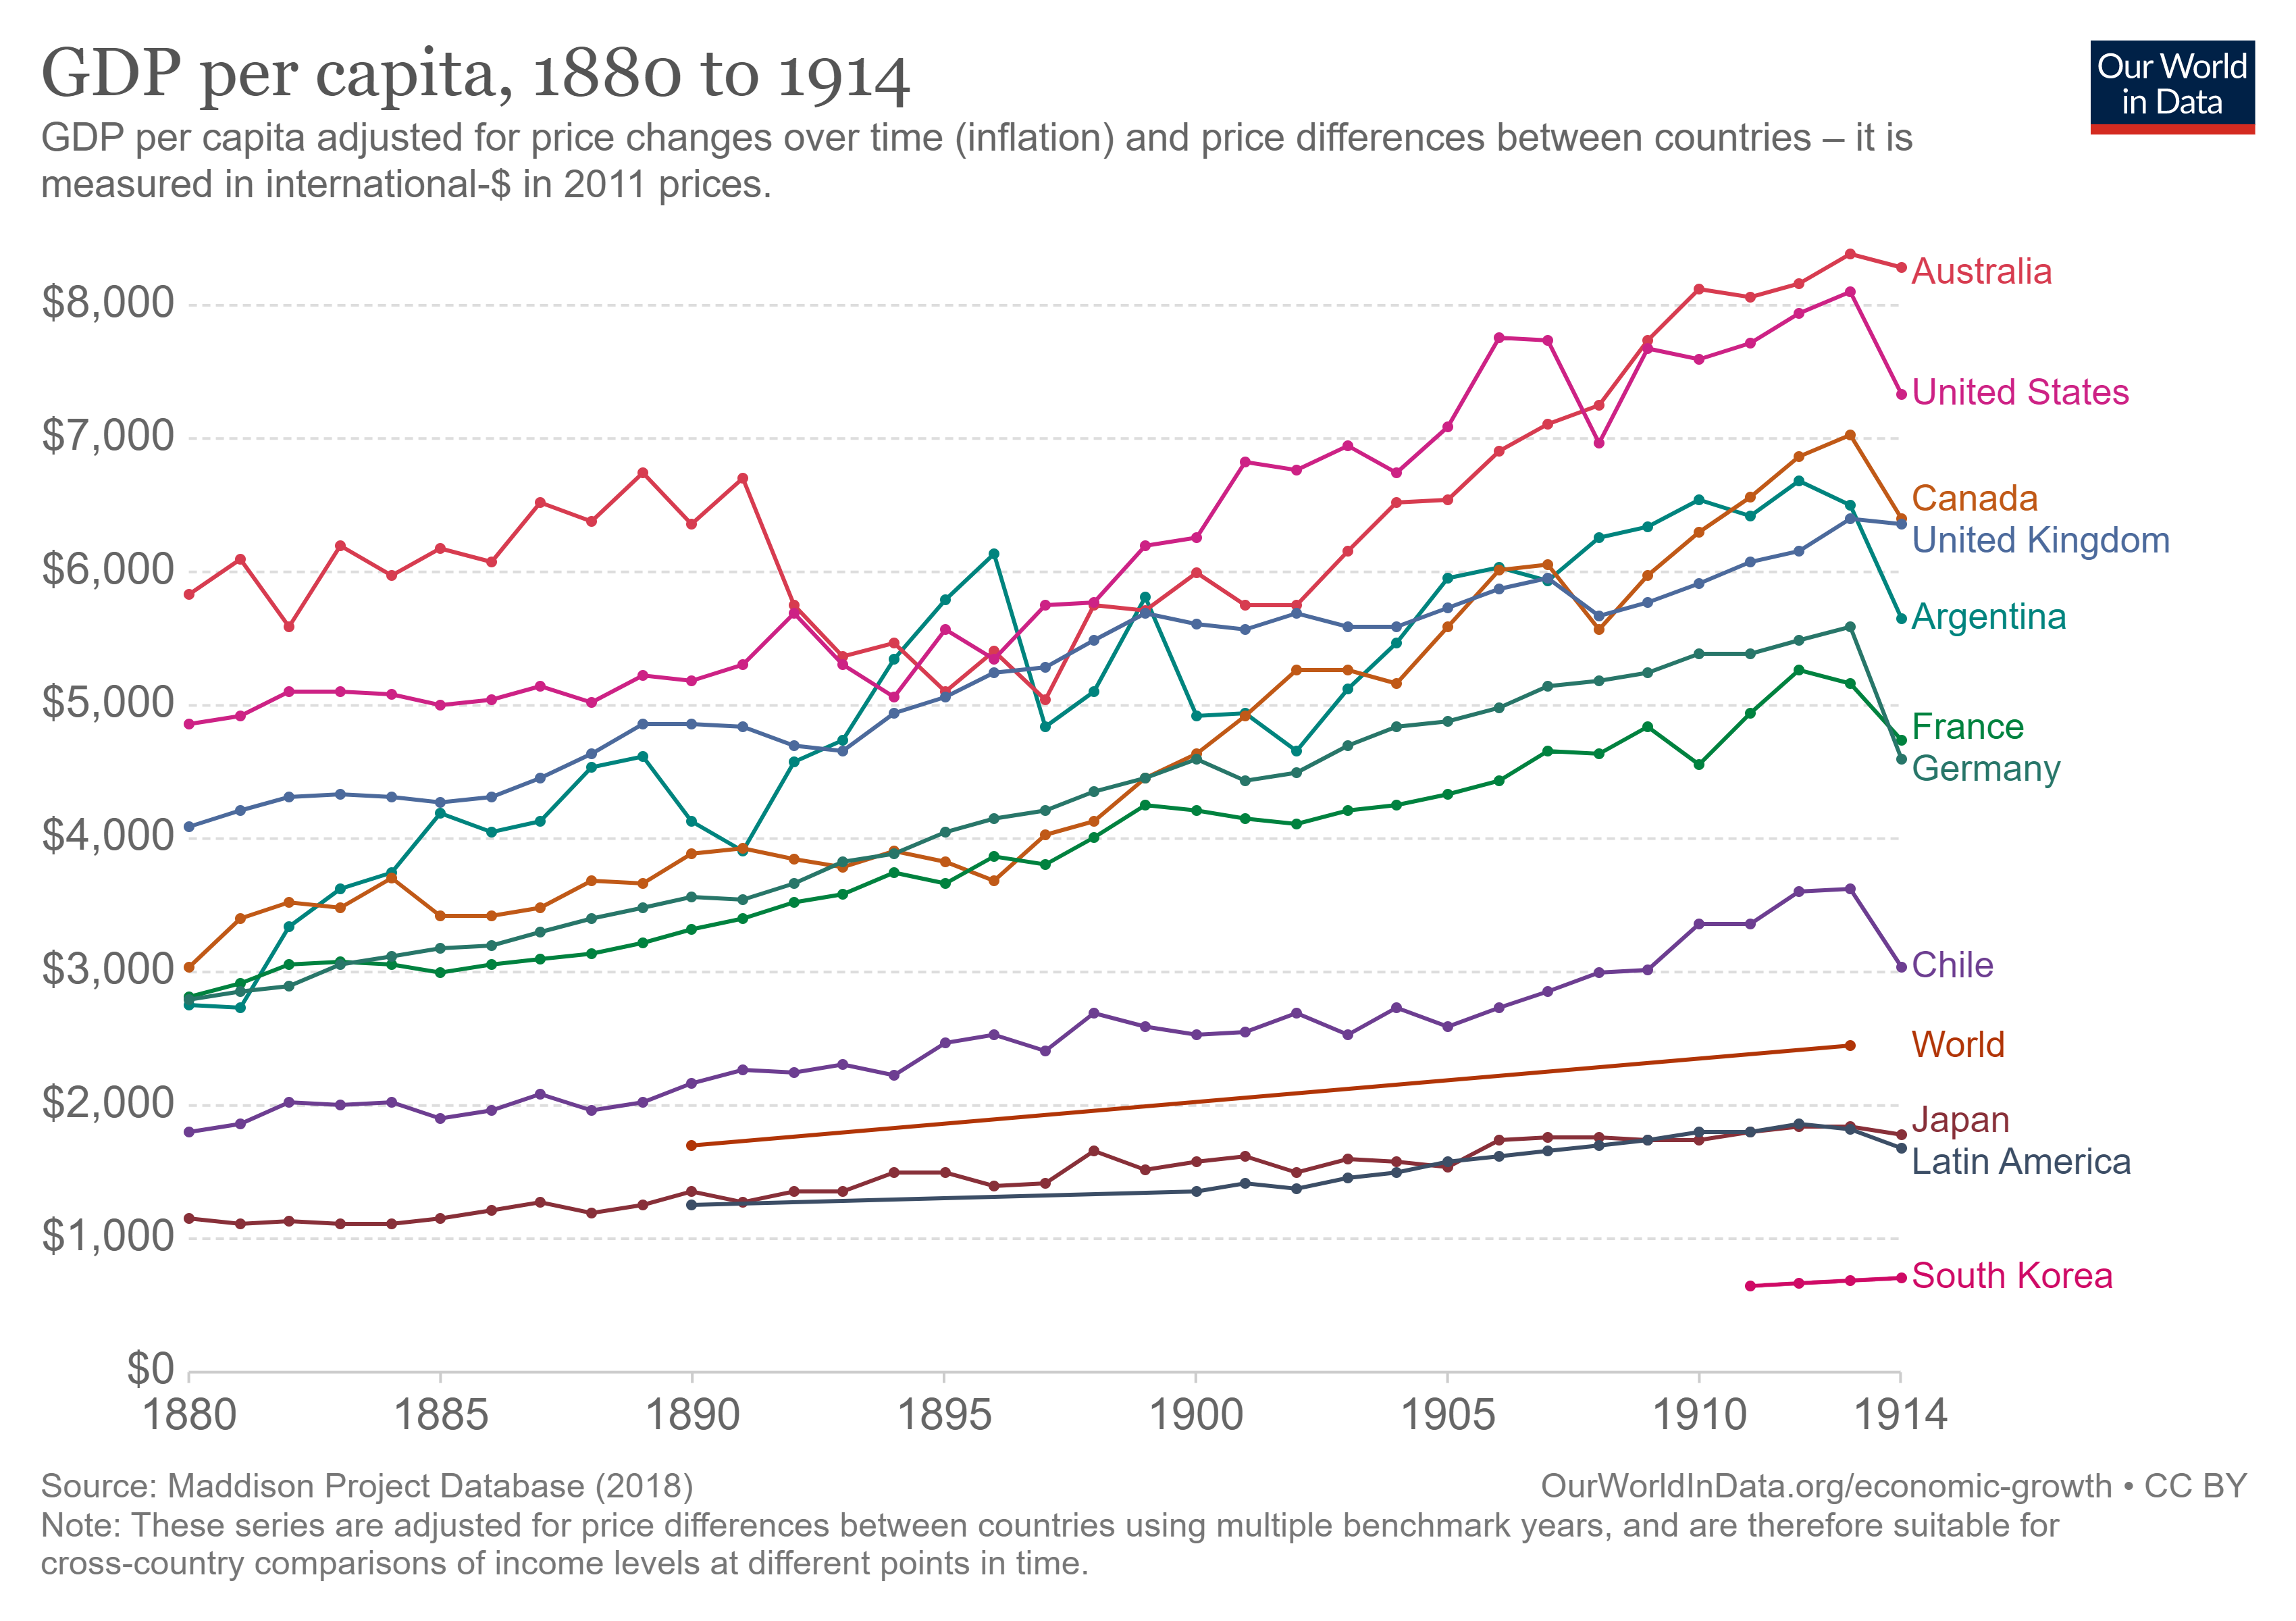
\includegraphics[scale=0.07]{maddison-data-gdp-per-capita-in-2011us-1880-1914}
        %\caption{Crecimiento argentino comparado: 1880-1914}
      \end{figure}
    \end{column}
  \end{columns}
  \end{frame}
  

\begin{frame}\frametitle{Teoría del bien primario exportable (BPE)}
  \begin{itemize}
    \item Teoría BPE atribuida a Innis (\textit{staple thesis}) para
      explicar crecimiento en Canadá y basada en dotaciones
      factoriales --abundancia de tierra y escasez de
      población. Ejemplos de uso la teoría BPE: North (1959, 1964,
      1991); Cortés Conde (1979, 1985, 1997).
    \item Es una teoría del crecimiento económico $\longrightarrow$
      crecimiento económico determinado por bienes primarios
      exportables.
      \item Inicialmente $\longrightarrow$ tierra (abundante), 
        trabajo (escaso) y  mercado interno (pequeño/inexistente)
        --exportaciones intensivas en factor tierra principal ventaja comparativa
       \end{itemize}
  \end{frame}


\begin{frame}\frametitle{Teoría del bien primario exportable (BPE) (cont.)}
  \begin{block}{Supuesto 1}
\textbf{Espacio vacío}, es decir, países nuevos
$\longrightarrow$ relación tierra/trabajo muy alta ($T/L$ y $T/K$) muy alta 
\end{block}
\begin{block}{Supuesto 2}
Dotación específica de recursos que asimile efectos del
crecimiento basado en exportación de primarios
$\longrightarrow$ efectos sobre estructura y distribución del ingreso
\end{block}
\begin{block}{Supuesto 3}
No existen tradiciones inhibidoras y/o restricciones institucionales $\longrightarrow$ limiten uso de recursos y/o tecnología
  \end{block}
  \end{frame}



\begin{frame}\frametitle{Teoría del bien primario exportable (BPE) (cont.)}
  \begin{block}{Dinámica}
    El argumento básico de la \textbf{staple theory} (teoría del bien
    primario exportable) es que los bienes primarios exportables son
    el sector líder de la economía y marcan el camino del crecimiento
    económico. El limitado -al principio posiblemente inexistente-
    mercado interno y la relativa abundancia de tierras respecto del
    capital y el trabajo, crea una ventaja comparativa favorable a las
    exportaciones de insumos o bienes primarios. El desarrollo
    económico será un proceso de diversificación en torno a una base
    exportadora... [Watkins (1963) en Gallo (1998)]
  \end{block}
  \end{frame}
  

\begin{frame}\frametitle{Teoría del bien primario exportable (BPE) (cont.)}
  \begin{block}{Dinámica}
    Inicialmente, es rentable exportar productos intensivos en
    tierra. El tipo de función de producción es unidad agrícola de
    tamaño familiar. Aparecen aqui los
    \textbf{eslabonamientos}. Por un lado, \textbf{eslabonamientos hacia atrás}
    como el desarrollo de un sistema de transporte y
    logística. Por otro, \textbf{eslabonamientos hacia adelante} en
    que el BPE es insumo de otro bien. Finalmente,
    \textbf{eslabonamientos de demanda final}, a través de producción
    de bienes de consumo final para los factores de producción de
    bienes exportables.  
  \end{block}
  \end{frame}


  
\begin{frame}\frametitle{Teoría del bien primario exportable (BPE) (cont.)}
\begin{figure}[htbp]\vspace{-0.1cm}
  \centering
  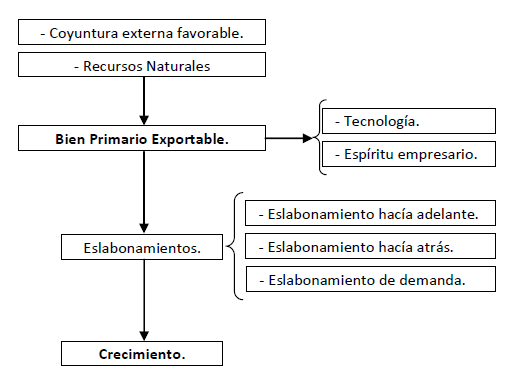
\includegraphics[scale=0.55]{uni1_bpe01}
  \caption[bpe]{Diagrama ilustrativo - Bien primario exportable}
  \label{fig:uni1_01}
\end{figure} 
  \end{frame}


\begin{frame}\frametitle{Teoría del bien primario exportable (BPE) (cont.)}
  \begin{itemize}
\item Importante distinguir entre: modelo de unidad agrícola familiar
  y modelo plantacion.
  \item En el primero, los eslabonamientos son más fuertes que en el
    segundo --modelo unidad agrícola familiar menos productivo por
    unidad de tierra y requiere mas servicios de transporte
    \item En el primero, ingreso está más equitativamente distribuido
      --efectos eslabonamientos de demanda final más homogéneos
    \end{itemize}
  \end{frame}


  \begin{frame}\frametitle{Teoría BPE: ¿Qué bien exportamos?}
  \begin{itemize}
  \item Elección de bien a exportar función varios elementos:
    \begin{enumerate}\itemsep 10pt \medskip
      \item De coyunturas externas $\longrightarrow$ variación de
        precios internacionales determina rentabilidades diferenciales
        \item De dotación de recursos naturales $\longrightarrow$
          tierra, minerales, y otros --mientras más diversificado,
          mas probable de aprovechar ciclos de precios favorables
        \end{itemize}
        \item Dos factores claves para poner en marcha el ciclo: 1)
          tecnología de producción; 2) espíritu empresarial
          \end{itemize}
  \end{frame}

\begin{frame}\frametitle{Teoría BPE: Eslabonamientos}
  \begin{itemize}
  \item El incentivo a la inversión interna como respuesta al
    crecimiento del sector exportador puede dividirse en:
    \begin{itemize}\itemsep 10pt \medskip
      \item \textbf{Eslabonamientos hacia atrás} $\longrightarrow$
        incentivo a invertir en insumos de producción local para el
        sector exportador (materias primas, bienes de capital)
        \item \textbf{Eslabonamientos hacia adelante}
          $\longrightarrow$ incentivo a invertir en industrias que
          utilizan como insumo el bien exportable
          \item \textbf{Eslabonamientos de demanda final}
            $\longrightarrow$ incentivo a invertir en industrias de
            producción de bienes de consumo destinados a factores
            empleados en el sector exportador
          \end{itemize}
\end{itemize}
        \end{frame}


\begin{frame}\frametitle{Teoría BPE: Eslabonamientos (cont.)}
  \begin{itemize}
  \item El nivel de PBI total será función del tamaño absoluto del sector
    exportador; el nivel de PBI per cápita será función de
    productividad de factores asociados al BPE
    \item Los eslabonamientos de demanda final serán mayores a mayor
      nivel de ingreso medio y mayor equidad distributiva --extremo
      inequidad completa bienes de lujo (importados) y bienes de
      subsistencia
      \item Crecimiento económico (cantidad y calidad)
        $\longrightarrow$ profundidades y tipos de eslabonamientos
        --eventual diversificación 
          \end{itemize}
        \end{frame}

        
\subsubsection{El caso de Argentina}

\subsubsection{Los bienes primarios exportables}

\begin{frame}\frametitle{Teoría BPE: Argentina}
  \begin{itemize}
  \item Los primeros bienes primarios exportables en Argentina (1776-1860)
    provenían de la \textbf{cría del ganado vacuno} $\longrightarrow$
    cuero, sebo y tasajo (carne salada) [productos no refinados]
    \item En 1860s importantes cambios debidos a factores externos
      (aumento $P^{*}$ lana) e internos (formación del
      Estado nacional) $\longrightarrow$ \textbf{cría del ganado
        ovino} --cambio función de producción (+ intensiva, + eslabonamientos)
      \item En 1880s se produce \textbf{el gran cambio} $\longrightarrow$
        coyuntura externa muy favorable --aumenda demanda
        internacional de carne [productos refinados]
          \end{itemize}
        \end{frame}
  


\begin{frame}\frametitle{Teoría BPE: Argentina (cont.)}
  \begin{table}[htbp]
    \centering
    \begin{tabular}[htbp]{lrrrr}\hline\hline 
      Producto & 1825 & 1854 & 1863 & 1873  \\\hline
      Cuero & 53.5 & 26.7 &  25.0  &  13.0  \\
      Sebo y grasas  & 32.0   & 26.7 &  21.4  & 17.4 \\
      Tasajo& 9.3  & 20.0   & 10.7 &  8.7 \\
      Lana  &  --    & 20.0  & 35.7 & 45.7  \\
      Piel de oveja & -- & -- & 3.6 & 10.9 \\
      Otros & 5.2  & 6.6 & 1.8  & 4.3  \\                              
                                \end{tabular}
    \caption{Composición exportaciones}
    \label{tab:table1}
  \end{table}
        \end{frame}
  



        \begin{frame}\frametitle{Teoría BPE: Argentina (cont.)}
  \begin{itemize}
     \item Sistema únicamente agrícola $\longrightarrow$ propietarios
      de tierras pequeñas/medias en zona litoral [colonización
      temprana]
      \item Combinación de usos (ganadería+agricultura) $\longrightarrow$
    lino, trigo y maíz/alfalfa --sistema de
    arrendamientos
    \item Mejores rendimientos en tierras no roturadas (sistema
      combinado y rotación de cultivos)
      \item Recién en 1890s, cambia la composición de X
        $\longrightarrow$ cereales en 26.1\%, carnes en 2.1\% lana
        33\%, y cueros 17\%; entre 1900-1914 cereales y carnes eran el
        54\% de las X. 
          \end{itemize}
        \end{frame}
  


  \begin{frame}\frametitle{Teoría BPE: Argentina (cont.)}
\vspace{-0.5cm}
    \begin{columns}
    \begin{column}{0.4\linewidth}
      \begin{itemize}
        \item Rezago entre el aumento en Q y aumento en X
        \item Tendencia ascendente
          \item Año de quiebre 1897-98 --boom exportaciones
      \end{itemize}
    \end{column}
    \begin{column}{0.6\linewidth}\vspace{-0.25cm}
      \begin{figure}
        \centering
        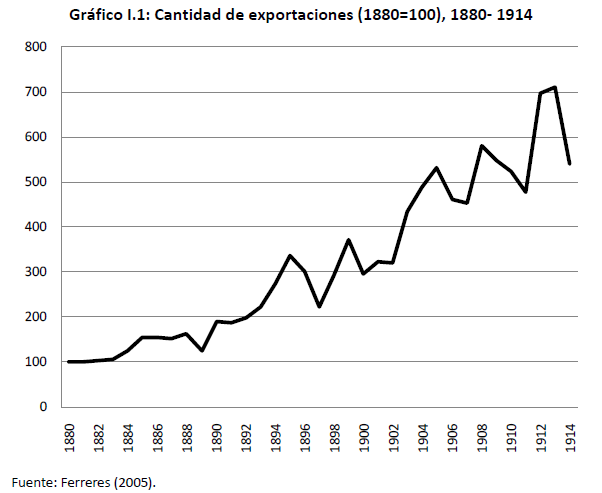
\includegraphics[scale=0.45]{uni1_bpe02}
        % \caption{Cantidad de exportaciones - Fuente: Gómez (2012)}
      \end{figure}
    \end{column}
  \end{columns}
\end{frame}


  \begin{frame}\frametitle{Teoría BPE: Argentina (cont.)}
\vspace{-0.5cm}
    \begin{columns}
    \begin{column}{0.4\linewidth}
      \begin{itemize}
        \item Serie similar en valor que a cantidad
        \item Tendencia ascendente
          \item Año de quiebre 1897-98 --boom exportaciones
      \end{itemize}
    \end{column}
    \begin{column}{0.6\linewidth}\vspace{-0.25cm}
      \begin{figure}
        \centering
        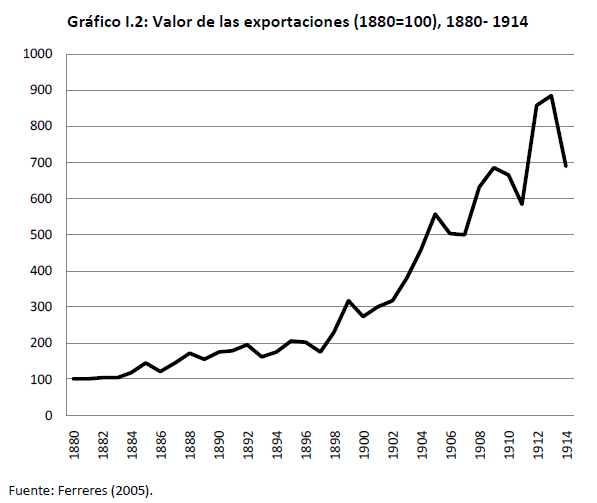
\includegraphics[scale=0.45]{uni1_bpe03}
        % \caption{Valor de exportaciones - Fuente: Gómez (2012)}
      \end{figure}
    \end{column}
  \end{columns}
  \end{frame}


  \subsubsection{Los factores productivos}


        \begin{frame}\frametitle{El caso argentino: Tierra}
  \begin{itemize}
     \item La tierra era abundante inicialmente (franja desde
       Mendoza hasta Buenos Aires y litoral); ampliado aún más luego
       de campaña del desierto (1880). Se anexan 30 millones de
       hectáreas (50\% mas)
       \item En este período la tierra se comportó atípicamente como
         un factor variable y no fijo --este gradual aumento de
         tierra cultivada contribuyó al aumento de X
         \item La superficie cultivada pasó de menos de 1 millón a
           casi 20 millones de hectáreas entre 1880 y 1912. 
          \end{itemize}
        \end{frame}


            \begin{frame}\frametitle{El caso argentino: Tierra (cont.)}
 \vspace{-0.5cm}
    \begin{columns}
    \begin{column}{0.6\linewidth}
 \begin{figure}
        \centering
        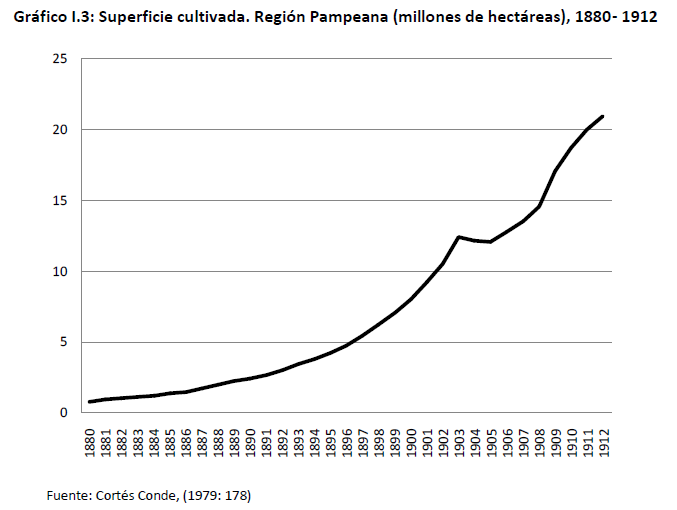
\includegraphics[scale=0.45]{uni1_bpe04}
        % \caption{Cantidad de exportaciones - Fuente: Gómez (2012)}
      \end{figure}
   
    \end{column}
    \begin{column}{0.4\linewidth}\vspace{-0.25cm}
     \begin{itemize}
     \item Fuerte y sostenido aumento de superficie cultivada
     \item Correlación con aumento en valor de X
       \item Lag de 2 años 
      \end{itemize}
    \end{column}
  \end{columns}
        \end{frame}
  

 \begin{frame}\frametitle{El caso argentino: Capital}
  \begin{itemize}
     \item La principal forma de \textbf{capital} en el siglo XIX
       fue el ferrocarril. Entre 1857 y 1914 se desarrollaron varias
       lineas y extensiones --Ferrocarril
       Oeste y el Ferrocarril Central Argentino (FCA) [Scalabrini
       Ortiz (1940)]
       \item La red ferroviaria creció de 2.4km a casi 35km entre 1880
         y 1914 aunque el ritmo de crecimiento no fue constante
         $\longrightarrow$ relación positiva con aumento de
         superficie cultivada
         \item Hubo algunas otras inversiones en infraestructura
           (puertos, riego) en gran mayoría financiadas con IED (casi 60\%). 
          \end{itemize}
        \end{frame}
        

   \begin{frame}\frametitle{El caso argentino: Capital (cont.)}
 \vspace{-0.5cm}
    \begin{columns}
    \begin{column}{0.6\linewidth}
 \begin{figure}
        \centering
        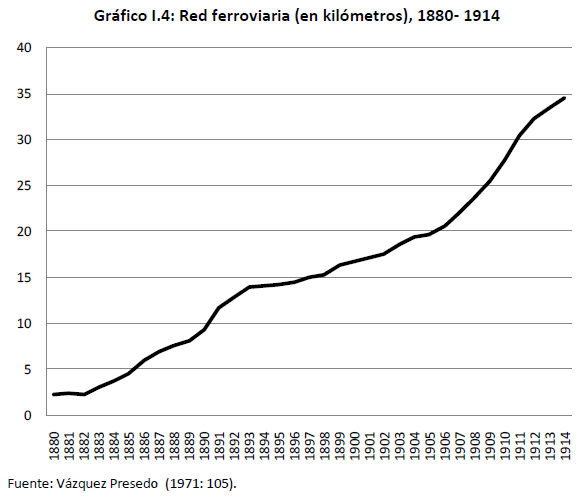
\includegraphics[scale=0.45]{uni1_bpe05}
        % \caption{Cantidad de exportaciones - Fuente: Gómez (2012)}
      \end{figure}
   
    \end{column}
    \begin{column}{0.4\linewidth}\vspace{-0.25cm}
     \begin{itemize}
     \item Ferrocarril rol central en crecimiento
     \item Trasladaba insumos y productos
       \item Lag de 1 y 11 años
      \end{itemize}
    \end{column}
  \end{columns}
        \end{frame}


        
\begin{frame}\frametitle{El caso argentino: Capital (cont.)}
\begin{figure}[htbp]\vspace{-0.1cm}
  \centering
  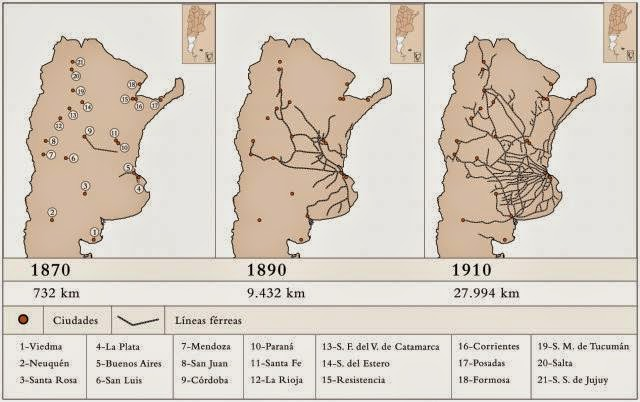
\includegraphics[scale=0.45]{uni1_bpe06}
  \caption[bpe]{Mapas - Red ferrocarriles argentinos}
  \label{fig:uni1_01}
\end{figure} 
\end{frame}

 \begin{frame}\frametitle{El caso argentino: Trabajo}
  \begin{itemize}
     \item De manera similar al capital, creció desde niveles muy
       bajos hasta lograr grandes aumentos en la dotación factorial
       --1.8 millones en 1869, 4 millones en 1895 y 7.9 millones en
       1914 $\longrightarrow$ influencia de inmigración
       \item Inmigración internacional gran responsable
         $\longrightarrow$ entre el 44\% y el 52\% del aumento de
         población en esos dos periodos
         \item Población inmigrante de dos países --Italia y
           España. Movilidad por diferencias salariales y por crisis
        en países de origen. 
          \end{itemize}
        \end{frame}


  \begin{frame}\frametitle{El caso argentino: Trabajo (cont.)}
 \vspace{-0.5cm}
    \begin{columns}
    \begin{column}{0.4\linewidth}
  \begin{itemize}
  \item Todo el período flujo neto positivo salvo crisis
  \item Casi 170 mil por año
    \item Mayor incidencia en PEA (edad laboral y  hombres)
       \end{itemize}
    \end{column}
    \begin{column}{0.6\linewidth}\vspace{-0.25cm}
           \begin{figure}
        \centering
        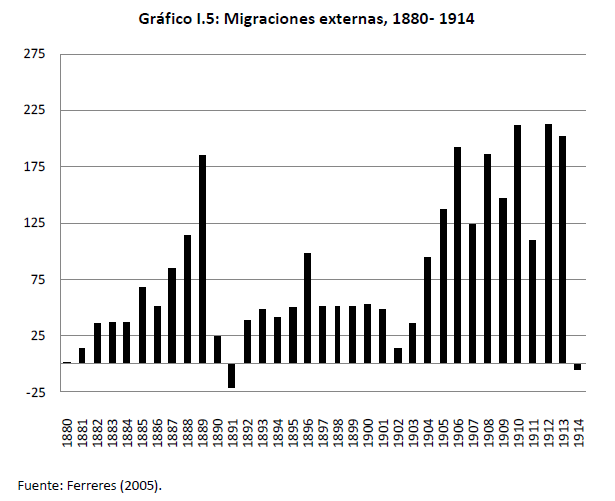
\includegraphics[scale=0.45]{uni1_bpe07}
        % \caption{Cantidad de exportaciones - Fuente: Gómez (2012)}
      \end{figure}
       \end{column}
  \end{columns}
        \end{frame}


\begin{frame}\frametitle{El caso argentino: Trabajo (cont.)}
  \begin{itemize}
     \item No hubo política inmigratoria nacional (como si hubo política de
       atraer IED) aunque si provincial
       \item Hubo además corrientes migratorias internas
         $\longrightarrow$ región pampeana receptora y noroeste, nordeste
         y cuyo emisoras [importancia secular de la región pampeana/litoral]
\item El aumento de la superficie cultivada estuvo directamente en
  relación con el aumento de la población rural [ver modelos]
       \end{itemize}
        \end{frame}
        

        
  \begin{frame}\frametitle{El caso argentino: Trabajo (cont.)}
 \vspace{-0.5cm}
    \begin{columns}
    \begin{column}{0.4\linewidth}
  \begin{itemize}
  \item Crecimiento promedio del 2\% entre 1880 y 1905
  \item Crecimiento promedio del 3\% entre 1905 y 1914
    \item Población rural eminentemente
       \end{itemize}
    \end{column}
    \begin{column}{0.6\linewidth}\vspace{-0.25cm}
           \begin{figure}
        \centering
        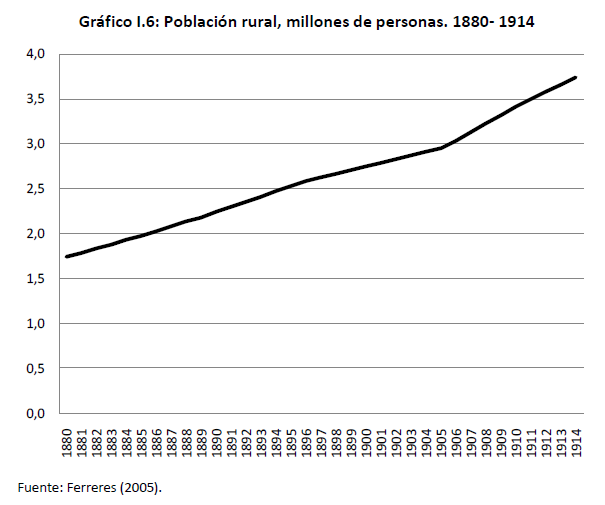
\includegraphics[scale=0.45]{uni1_bpe08}
        % \caption{Cantidad de exportaciones - Fuente: Gómez (2012)}
      \end{figure}
       \end{column}
  \end{columns}
        \end{frame}


  \subsubsection{La industria}


\begin{frame}\frametitle{Nacimiento de la industria: Decada de 1890}
  \begin{itemize}
     \item La fuerte expansión del sector rural agroexportador de
       finales de siglo XIX y principios de siglo XX tuvo impactos
       importantes en otros sectores
       \item Un primer efecto fue el impacto de los bienes exportables
         sobre el nacimiento de la \textbf{industria doméstica}.
         \item Estos efectos también permitieron la creación y el
           surgimiento del \textbf{mercado doméstico}.
           \item Efectivamente, dado que mercados regionales se
             integraron se puede hablar de un mercado único integrado
       \end{itemize}
        \end{frame}
  

\begin{frame}\frametitle{Nacimiento de la industria: Tipos de industria}
  \begin{itemize}
     \item Pueden clasificarse en 3 grandes grupos:
       \begin{itemize}\itemsep 10pt \medskip
       \item Primer grupo $\longrightarrow$  bienes
         transables; satisfacían demanda interna y externa; ventajas
         comparativas en el factor tierra; producto de los
         eslabonamientos hacia adelante [molinos harineros;
         frigoríficos]
         \item Segundo grupo $\longrightarrow$ bienes no transables;
           satisfacían demanda interna; sin ventajas comparativas;
           producto de eslabonamientos hacia atrás y de demanda
           [muebles; herramientas e instrumentos agrícolas; inmuebles]
           \item Tercer grupo $\longrightarrow$ bienes competidores de
             importaciones; satisfacían demanda interna; sin ventajas
             comparativas; producto de eslabonamientos de demanda
             [bebidas; vestimenta; químicos; fibras; tabaco] 
         \end{itemize}
       \end{itemize}
        \end{frame}

\begin{frame}\frametitle{Nacimiento de la industria: Crecimiento}
\begin{figure}[htbp]\vspace{-0.1cm}
  \centering
  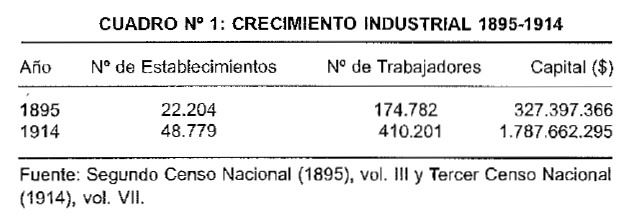
\includegraphics[scale=0.6]{uni1_ind01}
  \caption[bpe]{Evolución número de establecimientos. Fuente: Gallo (1998)}
  \label{fig:uni1_01}
\end{figure} 
\end{frame}


\begin{frame}\frametitle{Nacimiento de la industria: Crecimiento (cont.)}
\begin{figure}[htbp]\vspace{-0.1cm}
  \centering
  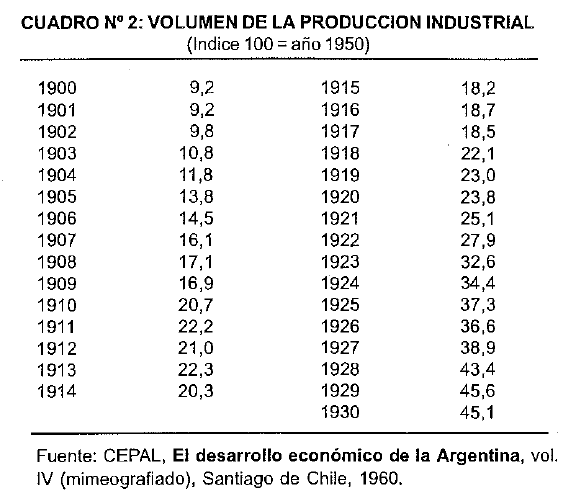
\includegraphics[scale=0.45]{uni1_ind02}
  \caption[bpe]{Evolución indice de producción industrial. Fuente:
    Gallo (1998)}
  \label{fig:uni1_01}
\end{figure} 
\end{frame}
        

        \begin{frame}\frametitle{Nacimiento de la industria: Características}
  \begin{itemize}
     \item Industria esencialmente orientada a satisfacer mercado
       interno no a exportaciones (2do y 3er grupo) --muy pocos rubros
       se exportaban (1er grupo).
       \item Número importante de empresas debía su existencia a
         \textit{factores de rentabilidad}
         \item Un factor era el \textbf{costo de
             transporte, $\tau$}
           $\longrightarrow$ casi el 70\% de las impor
           provenian de UK, Francia, Alemania y EEUU (grandes distancias
           daban cierta protección ``natural'')
           \item Otro factor era el \textbf{tipo de cambio, $E$}
             $\longrightarrow$ TC depreciado más protección
       \end{itemize}
        \end{frame}
  

     
           \begin{frame}\frametitle{Nacimiento de la industria:
               Rentabilidad}
  \begin{itemize}
     \item Finalmente, otro factor de rentabilidad es el
       \textbf{arancel a las importaciones, $t_{M}$}. En promedio en
       Argentina fue del 17.7\% en 1913, similar a EEUU y Canadá. 
     \item En otras palabras,
       \begin{equation*}
P_{d}=(P^{*}_{fob}+\tau)*E(1+t_{M})
\end{equation*}
\item Pero el arancel efectivo era mayor $\longrightarrow$ muchas
  importaciones exentas --RT sobre base imponible daba cercad e 30\%. 
       \end{itemize}
        \end{frame}



\begin{frame}\frametitle{Nacimiento de la industria: Rubros}
\begin{figure}[htbp]\vspace{-0.1cm}
  \centering
  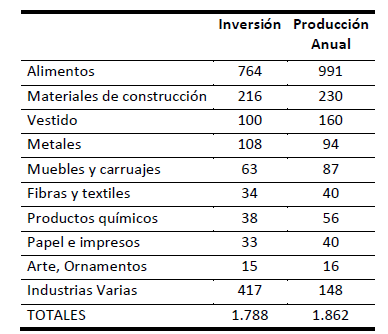
\includegraphics[scale=0.55]{uni1_ind03}
  \caption[bpe]{Valor de la producción y capital invertido
    (1914). Fuente: Gómez (2012)}
  \label{fig:uni1_01}
\end{figure} 
\end{frame}
        

 \begin{frame}\frametitle{Nacimiento de la industria:
               Rubros (cont.)}
  \begin{itemize}
     \item El principal rubro industrial eran los \textbf{alimentos}
       --principalmente la industria frigorífica, y los molinos
       harineros. Luego bastante más atrás seguía \textbf{materiales
         de construcción}. Los restantes grupos --metales; fibras y
       textiles; productos químicos- representaban menos del 5\%.
       \item La principal razón de porque no se desarrollaron estos
         últimos fue por la escasez relativa de hierro y carbón
         (metales); fuerte competencia inglesa (lanas/textiles);
         escasez de carbón y capital humano (productos químicos). 
       \end{itemize}
        \end{frame}


    \begin{frame}\frametitle{Nacimiento de la industria: Urbanización}
  \begin{itemize}
     \item La expansión de la industria trajo un aumento de la
       urbanización --población urbana pasó de 32\% en 1880 al 53\% en
       1914
       \item En todos los grandes centros urbanos --Buenos Aires,
         Rosario, La Plata y Córdoba- la población creció entre 2 y 3
         veces entre 1885 y 1914.
         \item Sin embargo, en 1900 la economia argentina era
           esencialmente una economía del bien primario --VA en sector
           agropecuario 85\% al VA del sector manufacturero; en 1914
           era casi un 60\% mayor.
       \end{itemize}
        \end{frame}
        



\begin{frame}\frametitle{Nacimiento de la industria: Urbanización (cont.)}
\begin{figure}[htbp]\vspace{-0cm}
  \centering
  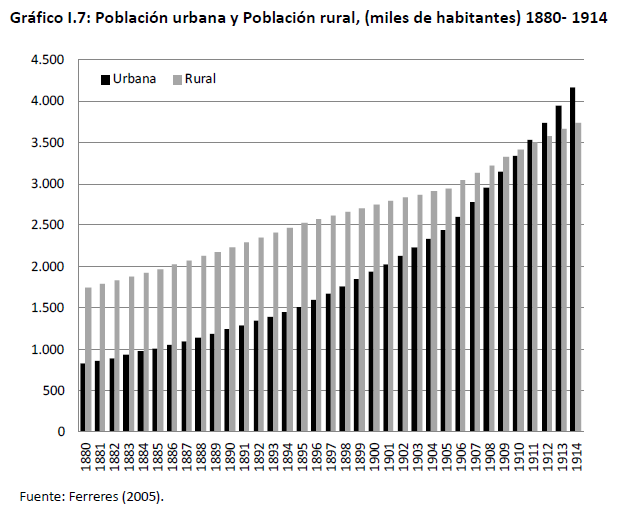
\includegraphics[scale=0.5]{uni1_urb01}\vspace{-0.5cm}
  \caption[bpe]{Población urbana y rural. Fuente: Gómez (2012)}
  \label{fig:uni1_01}
\end{figure} 
\end{frame}





\begin{frame}\frametitle{Nacimiento de la industria: Evolución}
\begin{figure}[htbp]\vspace{-0cm}
  \centering
  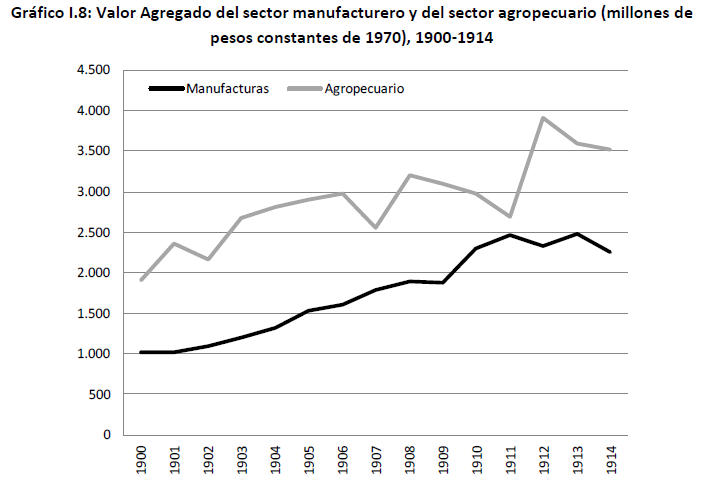
\includegraphics[scale=0.5]{uni1_urb02}\vspace{-0.3cm}
  \caption[bpe]{Valor agregado del sector manufacturero y
    agropecuario. Fuente: Gómez (2012)}
  \label{fig:uni1_01}
\end{figure} 
\end{frame}


  \begin{frame}\frametitle{Crecimiento ecónomico del período}
  \begin{itemize}
     \item Para poner en contexto el crecimiento económico argentino
       en este período es útil comparar con algunos países de mayor
       ingreso per capita del período: UK, Alemania, Francia, EEUU,
       Canadá y Australia. Por PBI per capita, Argentina ocupa el 5to
       lugar en 1913 (delante de Alemania y Francia)
       \item En terminos de ritmo de crecimiento, Argentina (2.5\%) está en el
         segundo lugar sólo detrás de Canadá (3.3\%) en el período
         1900-1913. 
       \end{itemize}
        \end{frame}


        
\begin{frame}\frametitle{Crecimiento económico del período (cont.)}
\begin{figure}[htbp]\vspace{-0cm}
  \centering
  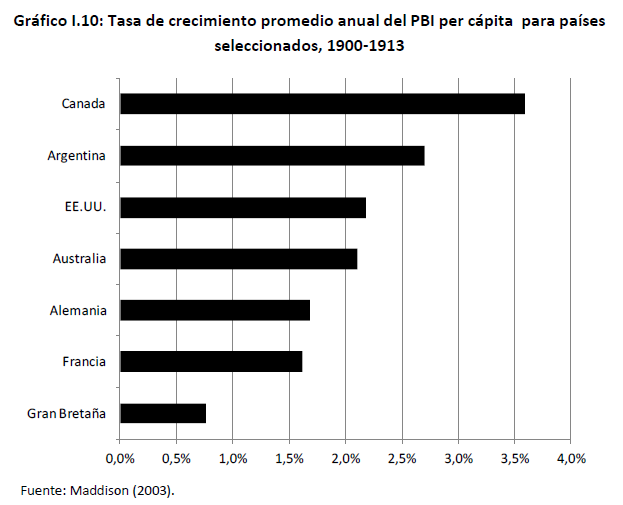
\includegraphics[scale=0.5]{uni1_growth01}\vspace{-0.4cm}
  \caption[bpe]{Tasa de crecimiento promedio anual, 1900-1913. Fuente: Gómez (2012)}
  \label{fig:uni1_01}
\end{figure} 
\end{frame}




\end{document}